%%%%%%%%%%%%%%%%%%%%%%%%%%%%%%%%%%%%%%%%%%%%%%%%%%%%%%%%%%%%%%%%%%%%%%%%%%%%%%%
\begin{frame}{MCNPX Simulations}
	\centering
	\begin{figure}
		
\includegraphics[width=0.25\textwidth]{logo-mcnpx.eps}
	\end{figure}
\begin{itemize}
    \item MCNPX is a well validated transport code \cite{pelowitz_mcnpx_2010}
    \begin{itemize}
        \item MCNPX is a Monte Carlo based
        \item MCNPX has drawbacks with energy deposition
    \end{itemize}
    \item Input decks based on pervious work (Martian Williamson)
    \item Many thanks to NE Cluster group for their support
\end{itemize}
\hyperlink{MCNPXMain}{\beamerbutton{Return to RPM Neutron Optimization}}
\hyperlink{toc}{\beamerbutton{Table of Contents}}
\end{frame}
%%%%%%%%%%%%%%%%%%%%%%%%%%%%%%%%%%%%%%%%%%%%%%%%%%%%%%%%%%%%%%%%%%%%%%%%%%%%%%%
\begin{frame}[fragile]
\frametitle{Gamma Irridiator Dose Rate}
	\tiny
	Need to create a 10 mR/hr field
	\newtheorem{MCNPXModelTHM10}{Dose Rate Calculation}
	\begin{MCNPXModelTHM10}<1->
		$$F2 = \frac{1}{A} \int_{A}{dA}\int_{E}{dE}\int_{4\pi}{d \Omega \Re(E) \Phi(\vec{r},E,\vec{\Omega})} $$
	where:
	\begin{itemize}
		\item $\Re(E)$ is the response function
		\item $\Phi(\vec{r},E,\vec{\Omega})$ is the photon flux
	\end{itemize}
	\end{MCNPXModelTHM10}
Accomplished using the DF Cards
\begin{lstlisting}
c Multiply each tally by 1000 mrem/rem * 100uCi * 3.7E10 Bq *2 photons / decay
FC12 Photon Flux over Front of Detector Surface
F12:P (500.2<600)
DE12  0.01 0.015 0.02 0.03 0.04 0.05 0.06 0.08 0.1 0.15 0.2 0.3 0.4 0.5 0.6  
		0.8 1 1.5
DF12  2.78E-6 1.11E-6 5.88E-7 2.56E-7 1.56E-7 1.20E-7 1.11E-7 1.20E-7 1.47E-7
      2.38e-7 3.45E-7 5.56E-7 7.69E-7 9.09E-7 1.14E-6 1.47E-6 1.79E-6 2.44E-6
\end{lstlisting}
\hyperlink{MCNPXMain}{\beamerbutton{Return to RPM Neutron Optimization}}
\hyperlink{toc}{\beamerbutton{Table of Contents}}
\end{frame}

%%%%%%%%%%%%%%%%%%%%%%%%%%%%%%%%%%%%%%%%%%%%%%%%%%%%%%%%%%%%%%%%%%%%%%%%%%%%%%%
\begin{frame}[fragile]
\frametitle{Interaction Rate}
	\tiny
	\newtheorem{MCNPXModelTHM11}{Interaction Rate}
	\begin{MCNPXModelTHM11}<1->
		$$Q = C \int {\Phi(E) R_m(E) dE }$$
	where:
	\begin{itemize}
		\item $C$ is a scalar normalization (density)
		\item $R_m(E)$ is the response function
		\item $\Phi(E)$ is the neutron flux
	\end{itemize}
	\end{MCNPXModelTHM11}
Accomplished using a F4 tally with multiplier
\tiny
\begin{lstlisting}
c -------------- Interaction Rate Tallies -----------------------
FC154 (n,t) Reactions in Detector in Pb Well
F154:n (601<610)
FM154 -1 3 105
FC214 Total Neutron Reactions in Detector in Cd Well
F214:n (601<620)
FM214 -1 3 1
\end{lstlisting}
\hyperlink{MCNPXMain}{\beamerbutton{Return to RPM Neutron Optimization}}
\hyperlink{toc}{\beamerbutton{Table of Contents}}
\end{frame}
%%%%%%%%%%%%%%%%%%%%%%%%%%%%%%%%%%%%%%%%%%%%%%%%%%%%%%%%%%%%%%%%%%%%%%%%%%%%%%%
\begin{frame}{Gamma Dose Rate Agreement}
\small
Compared simulated to measurements prefomed by RSO
	\begin{table}[h]
		\tiny
		\begin{tabular}{c c | c c}
        \multicolumn{2}{c}{Measured} & \multicolumn{2}{c}{Simulated} \\
        Distance (cm) & Dose Rate (mRem/hr) & Distance (cm) & Dose Rate (mRem/hr) \\
		\hline
		\hline
        10.2 & 10 & 10.2 & 10.3 \\
        13 & 5.5 & 12.7 & 5.38 \\
        28 & 2 & 28 & 1.80 \\
		\end{tabular}
	\end{table}
	\centering
	\begin{figure}
		\includegraphics[height=0.5\textheight]{DoseRate.eps}
		\caption{Dose Rate in Detector}
	\end{figure}
\hyperlink{MCNPXMain}{\beamerbutton{Return to RPM Neutron Optimization}}
\hyperlink{toc}{\beamerbutton{Table of Contents}}
\end{frame}
%%%%%%%%%%%%%%%%%%%%%%%%%%%%%%%%%%%%%%%%%%%%%%%%%%%%%%%%%%%%%%%%%%%%%%%%%%%%%%%
\begin{frame}{Neutron Simulation Agreement}
	Comparison between simulated neutron interaction rate and measured count rate. It is expected that some of the uncertainity in the fabricated samples comes from not knowing exactly the amount of \iso[6]{Li} in the film, as it is determined before casting or pressing.
  \small
\begin{table}
	\centering
	\label{tab:MCNPXVal}
	\begin{tabular}{m{3cm} | p{2cm} p{2cm} p{1cm}}
		\toprule
			Sample & Simulated Interaction Rate & Measured Count Rate & Relative Error \\
		\midrule
			GS20 & 424  & 428 & 0.7\%  \\ 
			PS 30\% LiF \SI{50}{\um} &  56 & 51 & 9.5\% \\
			PS 30\% LiF \SI{25}{\um} & 108 & 96 &13\%  \\
			PEN, 10\% LiF, \SI{110}{\um} & 75.1 & 70 & 7\% \\
			EJ426 HD2 & 226 & 224 & 0.8\% \\
		\bottomrule
	\end{tabular}
\end{table}
	\tiny
	\begin{definition}[Relative Error]
		$$\sigma = \frac{\text{Obs} -\text{ Sim}}{\text{Obs}}$$
	where:
	\begin{itemize}
		\item $\text{Obs}$ is the observed count rate
		\item $\text{Sim}$ is the simulated count rate
	\end{itemize}
	\end{definition}
\hyperlink{MCNPXMain}{\beamerbutton{Return to RPM Neutron Optimization}}
\hyperlink{toc}{\beamerbutton{Table of Contents}}
\end{frame}
